\documentclass[./thesis.tex]{subfiles}

\newcommand{\minDetInT}{\text{minDetInT1}}
\newcommand{\lTeethI}{\text{lTeethI}}

\begin{document}
\label{chap:PT2}

\section{Introduction}


In the literature, the computation of $\EPT$ is part of the CIPSI method. This is understandable, as the selection and the computation of $\EPT$ involve gathering the same data.
\begin{equation}
\EPT = \sum_\alpha \frac{\Hij{\Psi}{\alpha}^2}{\Delta E_\alpha}
\end{equation}
It is essentially the sum all $e_\alpha$ that are computed during a CIPSI selection.
\begin{equation}
\EPT = \sum_\alpha e_\alpha
\end{equation}
We have seen in section~\ref{sec:cipsi_approx} that approximate calculations could be done to accelerate the selection. However, these approximations don't apply to the computation of $\EPT$, so we designed a hybrid stochastic-deterministic scheme to get an accurate estimation of $\EPT$ for a much more reasonable cost. 


The selection of determinants and the calculation of $\EPT$, all approximations aside, both imply the computation of $e_\alpha$ for all $\ket \alpha$, so both can be computed at the same time. The selection is about identifying the set of the most important contributions, $\EPT$ is about computing the sum over all of them. There are two main consequences to this:
\paragraph{$\EPT$ is one iteration behind the selection}
At iteration $n$, identifying the most significant $\ket \alpha$ is about building $\ket {\Psi^{(n+1)}}$ while summing the contributions is about estimating the distance to full-CI for $\ket {\Psi^{(n)}}$. Computing $\EPT$ for a ``final'' wave function therefore requires an extra iteration, which applies to a larger number of determinants and thus is more expensive. Note that if only $\EPT$ is required, a more efficient algorithm can be used.\cite{Cimiraglia_1996}

\paragraph{The selection can take more approximations}
The computation of the sum has to be more costly than just identifying the largest terms. As was said in chapter~\ref{chap:CIPSI}, the CIPSI algorithm can take pretty drastic approximations for the selection.\cite{Evangelisti_1983}
	\begin{itemize}
		\item{$\Ngen$}
		allows to explore a reduced subset of $\ket \alpha$ in which we are almost sure to find those of interest.
		\item{$\Nsel$}
		allows for a less accurate and less expensive computation of $e_\alpha$, which is unlikely to significantly change the identified set.
	\end{itemize}
	These approximations do not apply when computing $\EPT$. The very large number of smaller contributions makes them impossible to neglect without introducing a bias, and increasing the $n_g$ and $n_s$ thresholds dramatically increases the computational cost.


Unfortunately, a truncated computation of $\EPT$ always yields in a biased result. Since $e_\alpha$ is the contribution to the correlation energy brought by $\kalpha$, it is necessarily negative. Hence, $\EPT$ is a sum of same-sign contributions, and when the sum of $e_\alpha$ is truncated some correlation energy is missing.
%The $n_g$ threshold used in CIPSI determining $\Ngen$ can be seen as a way of adjusting this truncation to reach a given computational cost.
%In the selection step, an additional approximation was made in the computation of $\Hij{\Psi}{\alpha}$, where the threshold $n_s$ determined the $\Nsel$ determinants which were considered. This approximation is another source of error in the calculation of $\EPT$.

Before the stochastic computation of $\EPT$ was implemented, our best choice was to set low values of $n_g$ and $n_s$ while performing the selection, and accept very approximate values for $\EPT$ for intermediate wave functions. Then, once the selection was completed, we would raise them just for a final, very expensive ``$\EPT$ only'' iteration. In fact, an exact computation with $\Ngen=\Nsel=\Ndet$ was often prohibitively long, so the final $\EPT$ was still biased, and the biases were not well controlled. The effect was particularly important when computing atomization energies, where the $\EPT$ values were much more approximate on the molecule than on the atoms.
A practical way to circumvent this problem was already proposed 20 years ago, by giving an extrapolation of $\EPT$ when $n_g$ goes to one.\cite{Angeli_1997} However, the algorithm we propose here has the advantage of giving an unbiased result within a statistical confidence interval.

\section{Stochastic estimation of $\EPT$}

We eventually solved the previously discussed problem by turning the bias into an error bar. The basic idea is that, instead of trying to get the largest possible chunk of contribution, we can randomly pick $e_\alpha$ contributions and make a Monte-Carlo estimate for the sum over all $\ket \alpha$. In this case, to avoid any bias we must set
\begin{equation}
\Ngen = \Nsel = \Ndet^\star
\end{equation}

with $\Ndet^\star$ the number of internal determinants with non-zero coefficient.
Not only the estimate will be unbiased and much closer to the actual $\EPT$, but we will have an estimate for the error. Because $\EPT$ is itself used as an approximation
\begin{equation}
\Evar + \EPT \simeq \EFCI,
\end{equation}
an error significantly smaller than the typical accuracy of $\Evar + \EPT$ \textit{vs} $\EFCI$ is certainly acceptable.
Drawing randomly external determinants would probably not be efficient enough to improve significantly
the computational time, so the algorithm we have designed is more convoluted.


\subsection{Monte-Carlo sampling}

We generally want to compute a quantity $F$ which may be expressed as the expected value of a function $f(x)$ with respect to a probability distribution function $p(x)$:
\begin{equation}
F = \int_{-\infty}^\infty f(x) p(x) \text{d} x
\end{equation}
with 
\begin{equation}
\int_{-\infty}^\infty p(x) \text{d} x = 1.
\end{equation}
When $X_i$ are samples randomly distributed according to $p$, 
\begin{equation}
\label{eq:sum_mc}
F = \langle f \rangle_p =  \lim_{M\rightarrow \infty} \frac{1}{M} \sum_{i=1}^{M} f(X_i)
\end{equation}
So if one is able to draw $M$ samples $X_i$ with probability $p(X_i)$, $F$ may be approximated as
\begin{equation}
\bar{F} = \frac{1}{M} \sum_{i=1}^{M} f(X_i)
\end{equation}

The \emph{Central Limit Theorem} states that when independent random variables are added together, their normalized sum tends to a normal distribution. The variance of this normal distribution, 
\begin{equation}
\sigma^2(F) = \lim_{M\rightarrow \infty} \frac{1}{M} \sum_{i=1}^{M} \qty( f(X_i) - F)^2,
\end{equation}
reflects the dispersion of the $X_i$.
For a finite number of samples, the variance can be estimated as
\begin{equation}
\bar{\sigma}^2(F) = \frac{1}{M-1} \sum_{i=1}^{M} \qty( f(X_i) - \bar{F})^2,
\end{equation}
and the 68.2\% confidence interval (statistical error) is $\bar{F} \pm \sqrt{\frac{\bar{\sigma}^2(F)}{M}}$.

The simplest way to compute $\EPT$ with a Monte Carlo algorithm is to express $\EPT$ as
\begin{equation}
\EPT % = \sum_{\alpha = 1}^{N_\alpha} \frac{ \Hij{\alpha}{\Psi}^2 }{\Evar - H_{\alpha \alpha} } 
= \sum_{\alpha = 1}^{N_\alpha} e_\alpha
= \frac{1}{N_\alpha} \sum_{\alpha = 1}^{N_\alpha} N_\alpha e_\alpha
= \langle N_\alpha\, e_\alpha \rangle
= \sum_{\alpha = 1}^{N_\alpha} p(\alpha) N_\alpha e_\alpha 
\end{equation}
with $p(\alpha) = 1 / N_\alpha$. This corresponds to a uniform sampling of the $\kalpha$ determinants.

The largest the variance of $e_\alpha$, the slowest the convergence. Changing the sampling can reduce the variance, and one can make the sampling optimal by choosing the probability density
\begin{equation}
p(\alpha) = \frac{e_\alpha}{\mathcal{N}}
\end{equation}
and computing
\begin{equation}
\EPT = \sum_{\alpha = 1}^{N_\alpha} p(\alpha) \times \mathcal{N}
\end{equation}
Unfortunately in this case, the normalization constant $\mathcal{N} =
\sum_\alpha e_\alpha = \EPT$, and this would require to know already
$\EPT$ before doing the calculation.

Choosing a probability density which can be computed very fast and which
approximates $e_\alpha / \EPT$ is expected to improve the convergence.
If one takes the expression of 
\begin{equation}
\EPT = \sum_\alpha e_\alpha = 
\sum_I \sum_J c_I c_J \qty( \sum_\alpha \frac{\Hij{D_I}{\alpha} \Hij{\alpha}{D_J}}{\Delta E_\alpha}), 
\end{equation}
one can remark that
\begin{enumerate}
\item As the determinants were selected with a CIPSI criterion, all the $e_\alpha$ are expected to be small. In this regime, all the $\Delta E_\alpha$ are expected to be large, and large enough to consider that $1/\Delta E_\alpha$ is almost constant.
\item 
when $I=J$, each contribution to $e_\alpha$ has a negative sign due to the denominator. But when $I \ne J$, the sum is a sum of terms with alternating signs, almost cancelling each other. Hence, the dominant term of the sum is the diagonal term
\begin{equation}
\sum_I c_I^2 \qty( \sum_\alpha \frac{\Hij{D_I}{\alpha}^2 }{\Delta E_\alpha}). 
\end{equation}
\item $\sum_\alpha \Hij{D_I}{\alpha}^2 / \Delta E_\alpha$ can be seen as the correlation
energy of determinant $\kI$, and this quantity is expected to be of the same order of magnitude among all the determinants. 
\end{enumerate}
Therefore, we propose to pack together contributions of $\alpha$ such that the random variable becomes 
a quantity $e_I$ indexed by $I$ instead of $\alpha$
\begin{equation}
e_I = \sum_{\alpha \in \mathcal{A}_I} e_\alpha
\label{eq:ei_to_alpha}
\end{equation}
and use as a probability distribution
\begin{equation}
p(e_I) = {c_I^2}.
\end{equation}

\subsection{Packing of $e_\alpha$ into elementary contributions $e_I$}

\begin{figure}[h!]
	\begin{center}
		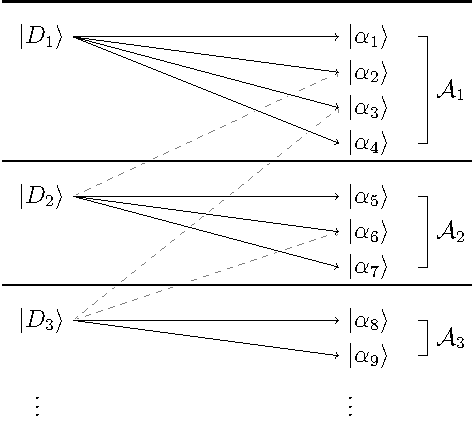
\includegraphics[width=0.5\columnwidth]{figures/pt2/a_sample}
	\end{center}
        \caption{Construction of batches of $\ket \alpha$: disjoint sets related to the generator determinant.}
        \label{fig:a_sample}
\end{figure}

Individual $e_\alpha$ are expensive to compute. In the CIPSI algorithm, each generator determinant creates a number of unique $\kalpha$, and computes $e_\alpha$ for each one of them.
Essentially, the set of $\kalpha$ is split in $\Ngen$ disjoint sets, each associated with a generator determinant, as shown in figure \ref{fig:a_sample}.
\begin{equation}
 \mathcal{A}_I = \left \{
e_\alpha \; ; \; \Hij{D_I}{\alpha} \neq 0 \; ; \;   \forall J < I, \Hij{D_J}{\alpha} = 0
\right \}.
\end{equation}
Because of the numerous tricks described in chapter~\ref{chap:CIPSI}, we are able to compute all the $e_\alpha$ of a set considerably faster than if we had to compute each contribution separately.
Fortunately, this partition of $\{ \kalpha \}$ fulfills the requirement of Eq.~\eqref{eq:ei_to_alpha}
and a large part of the implementation of the selection will be shared for the computation of the $e_I$
to make the stochastic computation of $\EPT$ efficient.

To draw samples distributed with $p(e_I)$, we use the \emph{inverse transform sampling method}.\cite{Devroye2013Nov}
The representation we are going to use is a collection of $\Ndet$ boxes of width $w_I$, containing the determinant of index $I$.
The determinant index $I$ associated with drawing a random number $u \in [0,1)_\mathbb{R}$ is noted $w[u]$. It is determined using the cumulative probability distribution function $W$
\begin{align}
W_I &= \sum_{J \leq I} w_J \\
w(u)& = I \; ; \; W_{I-1} \leq u < W_I.
\end{align}
To sample with $p(e_I)$, we set $w_I = p(e_I)$.

\begin{figure}[h!]
	\begin{center}
		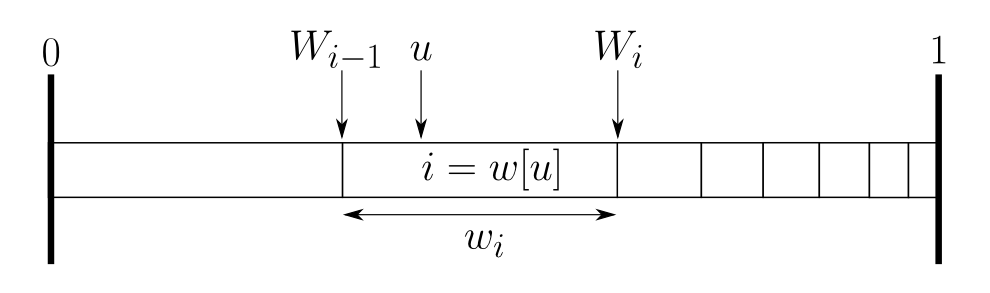
\includegraphics[width=0.7\columnwidth]{figures/pt2/mc_representation}
	\end{center}
	\caption{Schematic representation of 
Values inside the boxes are generator indices. Values outside are probabilities and drawn random numbers.
Drawing the random number $u$ using the probability density $w$ yields generator index $I=w(u)$.}
	\label{fig:mc_representation}
\end{figure}

\begin{figure}[h]
	\begin{center}
		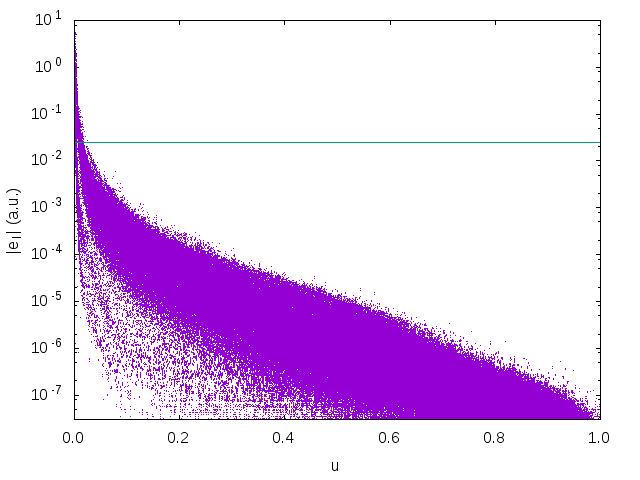
\includegraphics[width=0.49\columnwidth]{figures/pt2/eI}
		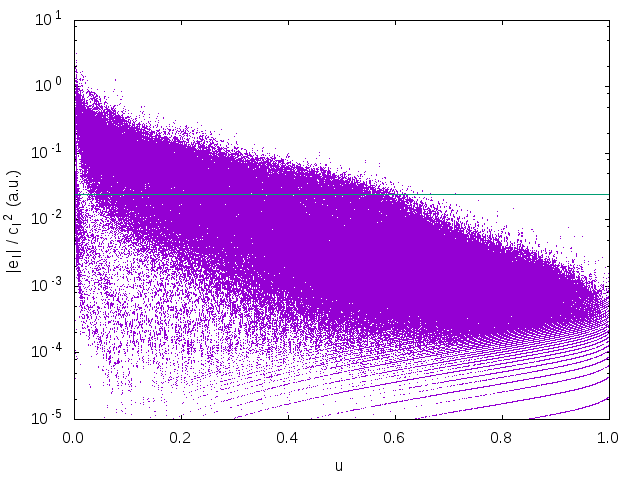
\includegraphics[width=0.49\columnwidth]{figures/pt2/eici2}
	\end{center}
		\caption{Contribution $|e_I|$ (left) and $|e_I|/c_I^2$ (right) as a function of the uniform random number $u$ drawn. The green horizontal line is $\EPT$.}
		\label{fig:ei}
\end{figure}
Figure~\ref{fig:ei} confirms that using $p(e_I) = c_I^2$ as a probability density gives less
fluctuations in the samples than when using a uniform sampling. The decreasing aspect of the curve
comes from the elimination of the duplicate $\kalpha$, which makes the $e_I$ smaller and smaller with respect to
the correlation energy of $\kI$.


To simplify the implementation, the actual distribution $w_I$ we use isn't exactly $c_I^2$. This will be detailed in section~\ref{sec:pt2_distribution}.



\subsection{Memoization of $e_I$'s}

Each contribution is now associated with a generator determinant. As a consequence, there are only $\Ngen$ elementary contributions to compute, but the computational cost of each contribution is increased.
The number of contributions is small enough to make all the $e_I$'s fit in memory, so when a $e_I$ contribution is computed, its value is stored and simply reused if the same generator is drawn again. This optimization technique is known as \emph{memoization},\cite{Michie1968Apr} and can make exponentially-scaling algorithms become polynomial.\cite{Frost1994}

In our case, this optimization also leads to a drastic improvement in the computational time: it takes an infinite time for a Monte Carlo calculation to reach a zero statistical error, but using the memoization technique the exact result will eventually be known in finite time, once every contribution has been computed. The cost for the exact computation will essentially be the same as that of the purely deterministic full computation, with a negligible additional cost due to the Monte-Carlo related computations (drawing random numbers, finding the associated generators\dots).



\section{Deterministic and stochastic ranges}
Because $e_I$ decreases rapidly, most of the contribution is contained in the first few $e_I$. We can compute the exact energy contribution for the first $e_I$, and only make a stochastic estimation for the sum over the smaller ones. This effectively splits the space of generators in two ranges, a deterministic one $\mathcal{D}_D$, then a stochastic one $\mathcal{D}_S$ (hence the hybrid characteristic of this method). Being ranges, they are always made of contiguous generators. The estimated energy can be written as
\begin{equation}
\EPT = E_D + E_S
\end{equation}
with $E_D$ the exact energy for $\mathcal{D}_D$, and $E_S$ the estimated energy for $\mathcal{D}_S$. The error bar only applies to $E_S$, which is typically much smaller than $E_D$.
The number of generators in $\mathcal{D}_D$ increases during the computation. Initially, $\mathcal{D}_D=\mathcal{T}_0$ the initial deterministic range, for which the total weight is $u_0$.
\begin{equation}
\sum_{I \in \mathcal{T}_0} w_I=u_0
\end{equation}
$\mathcal{T}_0$ is always computed before any stochastic estimation can take place.

\subsection{Partition of the stochastic range in $\Nteeth$ \emph{teeth}}
\label{sec:partition}

\begin{figure}[h!]
	\begin{center}
		\includegraphics[width=0.9\columnwidth]{figures/pt2/eici2_comb}
	\end{center}
	\caption{Contribution $e_I$ associated with each generator, where the generators are sorted in decreasing order of $c_I^2$. The determinant space is divided into equal probability ranges, according do $c_I^2$.}
	\label{fig:p_i}
\end{figure}

Generator determinants are sorted with decreasing values of $c_I^2$.
As can be seen in figure \ref{fig:ei}, the values of $e_I$ span many orders of magnitude and decrease rapidly with $I$, in an exponential-like way. Smoothed values for $e_I$ are shown in figure \ref{fig:p_i}. There are a few reasons for that.
\begin{itemize}
	\item
	The values for the denominator $\Delta E_\alpha$ used in the computation of $e_\alpha$ tend to increase, as internal determinants tend to be more and more excited and to populate higher orbitals 
	\item
	The number of unique $\ket \alpha$ per generator decreases. Indeed, the higher $I$, the likelier it is that the external determinants were were generated by other generators in $\{\ket{D}_{J<I}\}$.
	\item
	Unique $\ket \alpha$ are, by construction, disconnected from all previous generators, which mean they connect to a set of selectors with a decreasing norm.
\end{itemize}


Because of its original nature, this algorithm casts some ambiguity on what should be referred to as a \emph{sample}. We are going to estimate a sum of elementary contributions $e_I$, compute and store them individually, and draw them based on a probability distribution function ; therefore they will be referred to as the \emph{samples} and shown as such in the previously introduced representation. But the actual sample values are sums over several $e_I$, referred to as \emph{combs}.

\begin{figure}[h!]
	\begin{center}
		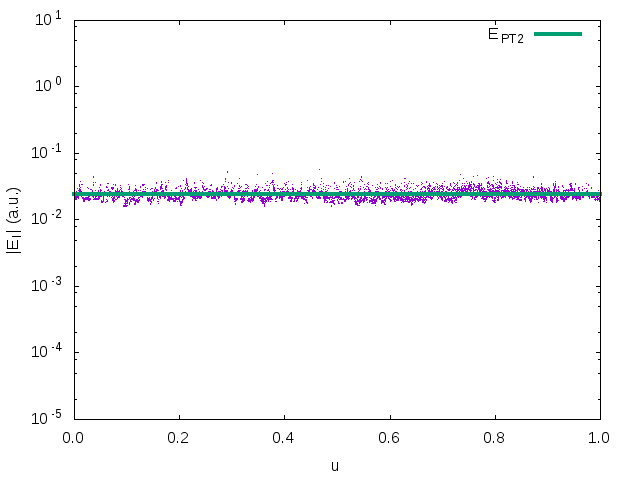
\includegraphics[width=0.7\columnwidth]{figures/pt2/comb_variance}
	\end{center}
		\caption{Comb contributions as a function of the uniform random number $u$ drawn. The green horizontal line is $\EPT$.}
		\label{fig:ei_comb}
\end{figure}
In a comb, the space of generators, minus the initial deterministic range $\mathcal{T}_0$, is split into ranges of equal probability (see
ranges $\mathcal{T}_1, \dots \mathcal{T}_4$ in figure~\ref{fig:p_i}), and
one sample is drawn in each range. Then, all those $e_I$ are added together to make the contribution of the comb. Because the function $e_I$ decreases smoothly, the contributions of the combs fluctuate less than the individual contributions, and the variance can be further reduced, as shown in figure~\ref{fig:ei_comb}.

As seen in section~\ref{sec:partition}, because $\frac{e_I}{w_I}$ overall decreases, a range has a lower variance than the whole domain. The stochastic range is split in $\Nteeth$ ranges referred to as \emph{teeth}, noted $\mathcal{T}_1,\ldots,\mathcal{T}_{\Nteeth}$ (called $\mathcal{D}_t$ in the presented article) and sharing the same total weight $W_T$
\begin{equation}
\sum_{I \in \mathcal{T}_{t \geq 1}} w_I=W_T.
\end{equation}

 \begin{figure}[h!]
	\begin{center}
	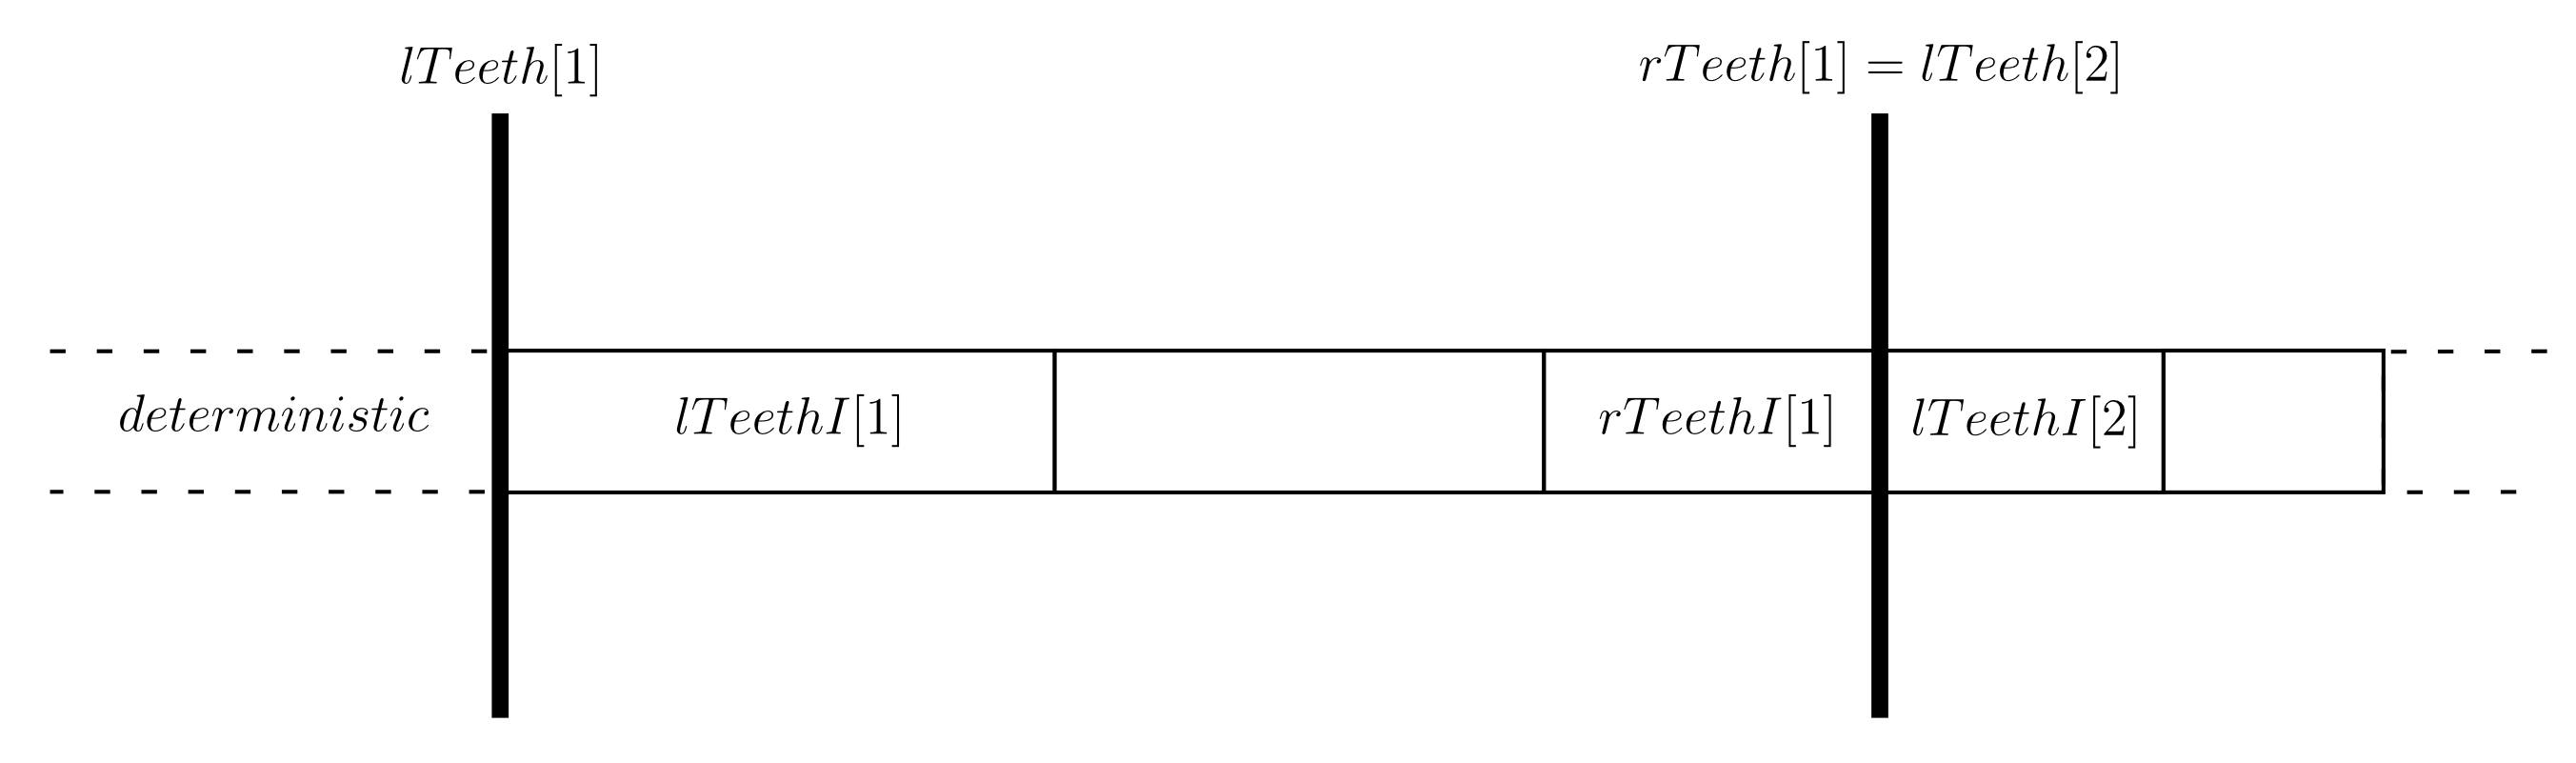
\includegraphics[width=0.6\columnwidth]{figures/pt2/teeth}
	\end{center}
	\caption{Partitioning of the generator space.
		The generator space is partitioned in so-called \emph{teeth} from $\mathcal{T}_0$ to $\mathcal{T}_{\Nteeth}$, $\mathcal{T}_0$ of total weight $u_0$, the others of total weight $W_T$}
	\label{fig:teeth}
\end{figure}

The partition of the generator space is as shown in figure~\ref{fig:teeth}.
Intuitively, the sum of ``one large, one medium and one small'' has a lower variance than the sum of ``three at random''. Instead of drawing individual indices, we are going to draw ``combs'' of indices, which are correlated sets of 1 index from each tooth. The associated sample value is the sum of $\frac{e_I}{w_I}$ over those indices that are in $\mathcal{D}_S$.  The expression for this sample value is given below in Eq.~\eqref{eq:combvalue}.

\subsection{Fully-computed teeth are moved to the deterministic range}

Remembering we store $e_I$, given the first tooth $\mathcal{T}_t$ that contains an unknown $e_I$, the deterministic range extends to all $\mathcal{T}_{p<t}$. This makes $\mathcal{T}_t$ the first non-deterministic tooth.
The number or generators in the deterministic range, therefore, is function of a tooth index $t$, and noted $n_0(t)$, as seen in figure \ref{fig:boundaries_teeth}

\begin{figure}[h!]
	\begin{center}
		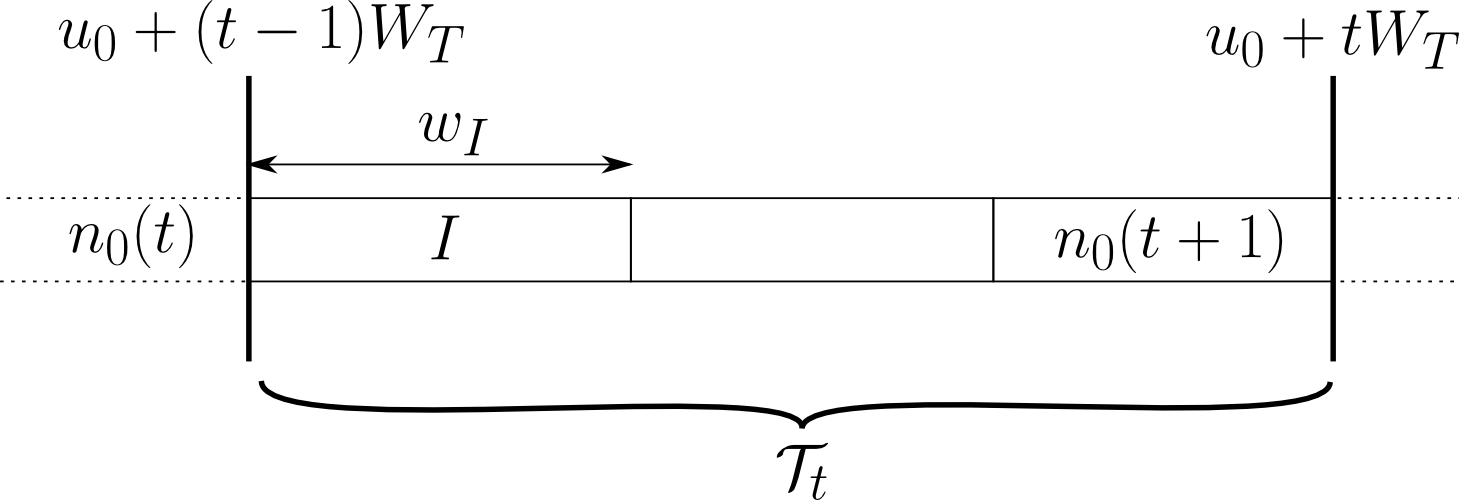
\includegraphics[width=0.7\columnwidth]{figures/pt2/tooththreshold}
	\end{center}
	\caption{Boundaries of a tooth index-wise and probability-wise}
	\label{fig:boundaries_teeth}
\end{figure}


\paragraph{Comb values}

We can write the expression of $B_t(u)$ the sample value associated with a comb. It is function of a random number $u \in [0,1)_\mathbb{R}$ and $t$ the index of the first non-deterministic tooth.

\begin{align}
\label{eq:combvalue}
B_t(u) = W_T \sum_{i=t-1}^{\Nteeth-1} \frac{e_{y(u+i)}}{w_{y(u+i)}} \\
y(x)=w[u_0+ W_T \times x, W]
\end{align}

An illustrative example is given as figure \ref{fig:toothindet}.

 \begin{figure}[h!]
	\begin{center}
		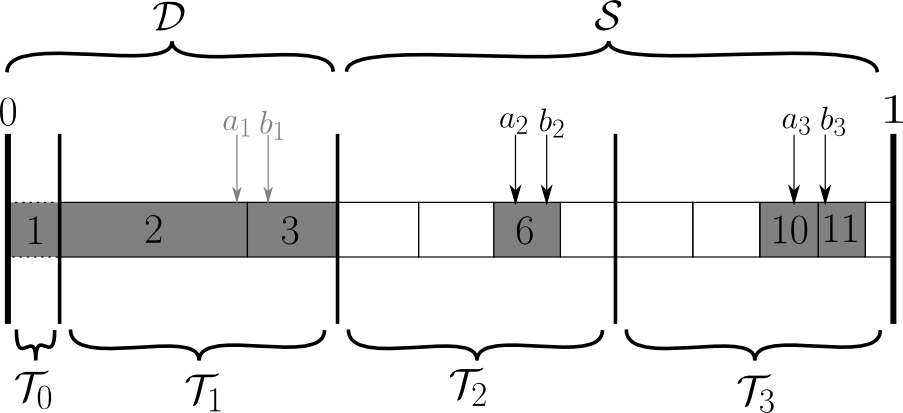
\includegraphics[width=0.75\columnwidth]{figures/pt2/toothindet}
	\end{center}
		\caption{Illustrative example of drawing $n=2$ combs $a$ and $b$. Contributions that have been computed are greyed. $\mathcal{T}_1$ has been fully computed and is thus moved to $\mathcal{D}_D$. The first non-deterministic/not fully-computed tooth is $\mathcal{T}_{t=2}$.
		$ E_D = e_1 + e_2 + e_3 $, 
		$B_t(a) = W_T \Big ( \frac{e_6}{w_6} + \frac{e_{10}}{w_{10}} \Big ) \;;B_t(b) = W_T \Big ( \frac{e_6}{w_6} + \frac{e_{11}}{w_{11}} \Big )$, 
		$E_S = \frac{B_t(a)+B_t(b)}{n}$}
		\label{fig:toothindet}
\end{figure}

\paragraph{Estimation of $\EPT$}

After drawing $n$ random numbers forming the set $\{\mathcal{U}\}$, and given $\mathcal{T}_t$ the first non-deterministic tooth, $\EPT$ can be estimated as 

\begin{equation}
\EPT = \sum_{I=1}^{n_0(t)} e_I + \frac{S_{t}}{n}  \pm \text{err}
\end{equation}
where the error is given by
\begin{equation}
\text{err}  = \sqrt{\frac{S_{t}^{(2)} - {S_{t}}^2}{n-1} } 
\end{equation}
\begin{align}
S_{t} & = \sum_{u \in \{\mathcal{U}\}} B_{t}(u) & 
S^{(2)}_{t} = \sum_{u \in \{\mathcal{U}\}} B_{t}(u)^2
\end{align}


\section{Technical considerations}


\subsection{Point of the initial deterministic part}

The initial deterministic range $\mathcal{T}_0$ is a technical constraint.
Because generators are sorted with decreasing $p(e_I)$, it is guaranteed that $|\mathcal{T}_{t>t'}| \geq |\mathcal{T}_{t' \neq 0}|-1$ with $|\mathcal{T}_t|$ the cardinality of $\mathcal{T}_t$.
For each comb, we draw a sample in each tooth, and when a tooth is entirely computed, it is moved to $\mathcal{D}_D$. Thus, it is immediately obvious that a tooth containing a single generator makes no sense, as it will be instantly moved to $\mathcal{D}_D$ ; it can as well be considered part of it. Because it is common practice to require at least 30 samples for the distribution of the average to become close enough to a Gaussian distribution,\cite{Hogg2014Jan} we can go further and consider that a tooth with fewer than 5-10 generators will be moved to $\mathcal{D}_D$ too fast to be of real interest. Because the first $c_I^2$ are usually disproportionately large, it is not possible to fit that many in a tooth. Therefore they are immediately considered part of $\mathcal{D}_D$.

\subsection{Desired \textit{vs} effective distribution function}
\label{sec:pt2_distribution}

We have defined all teeth (except the special $\mathcal{T}_0$) as sharing the same total weight $W_T$. This is a constraint on our desired distribution function $p(e_I) = c_I^2$ that will lead to the effective distribution function $w_I$.

We are sampling comb values, but we have defined $p(e_I)$ a distribution function for $e_I$. Since we impose that the same number of $e_I$ are drawn in each tooth ---~one per comb~--- the relative weight of teeth becomes irrelevant, and we effectively give all teeth the same weight 
\begin{equation}
W_T=\frac{1-u_0}{\Nteeth}
\end{equation}
in the Monte-Carlo scheme. Therefore, the effective weight given to $I \in \mathcal{T}_t$ is
\begin{equation}
w_{I \in \mathcal{T}_t} = W_T \times \frac{p(e_I)}{\sum_{J \in \mathcal{T}_t} p(e_J)}
\end{equation}

To leave the distribution function unaltered, we need all teeth to actually weigh $W_T$
\begin{equation}
\sum_{J \in \mathcal{T}_t} p(e_J) = W_T.
\end{equation}

Clearly this is not going to be the case for any distribution function $p(e_I)$. Schematically, as seen in figure \ref{fig:toothbuilding}, it would require the boundary between two teeth to exactly match the boundary between two generators. It is possible to artificially split in two a generator to get a matching boundary, but this adds some complexity in the implementation.

We have enforced that all teeth contain at least $5-10$ generators and they usually contain a lot more, up to hundreds of thousands. Therefore, a simpler solution is to ``round'' the teeth boundaries to the $e_I$ thresholds directly above, which will result in teeth with weights close to $W_T$, and thus the effective distribution function will be little different from the desired one. Since our distribution function is an extremely rough estimation of $e_I$, this is unlikely to cause any significant change in the convergence rate.

Essentially, we will use $p(e_I)$ only to define the $\mathcal{T}_t$ sets, then use $w$ as the actual distribution function. This gives us, by definition, teeth weighing exactly $W_T$.
This is illustrated in figure \ref{fig:toothbuilding}.
 
\begin{figure}[h!]
	\begin{center}
		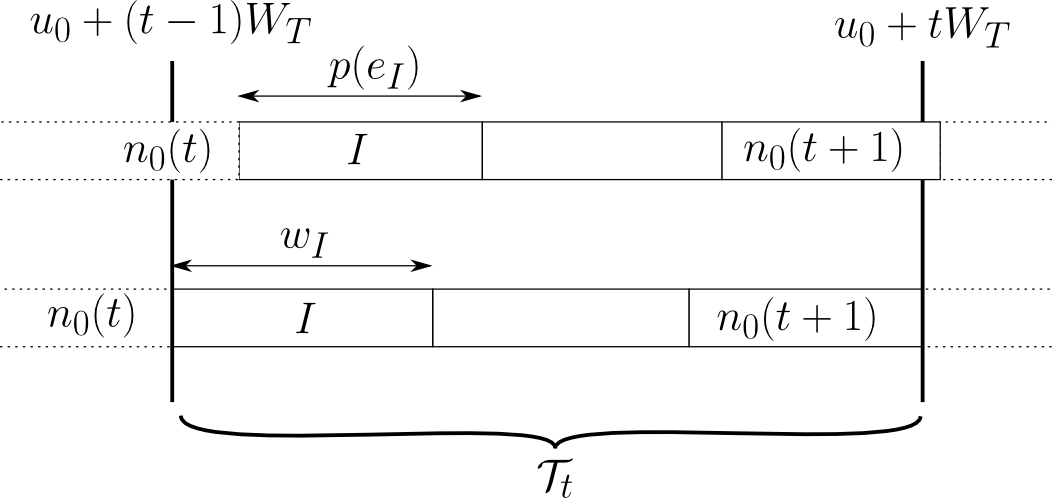
\includegraphics[width=0.9\columnwidth]{figures/pt2/toothbuilding}
	\end{center}
	\caption{Modifying $p(e_I)$ such that the boundaries of the teeth match with the boundaries of the generators, and so as to satisfy $\sum_{I \in \mathcal{T}_{t \neq 0}} w_I = W_T$.}
        \label{fig:toothbuilding}
\end{figure}





\subsection{Tooth filling}

This is an empirical mechanism to balance the stochastic and deterministic aspect of this method. For a tooth containing $n$ generators of equal probability, full computation is achieved after on average
\begin{equation}
\sum_{i=0}^{n-1} \frac{n}{n-i}
\end{equation}
combs are drawn. Thus, teeth containing thousands of determinants are very hard to move to $\mathcal{D}_D$. A tooth containing $10~000$ generators with a single non-computed contribution only needs that particular generator to be drawn in order to be moved to $\mathcal{D}_D$, but it will take on average $10~000$ more combs to be drawn until this happens by chance. With the non-uniform sampling, the situation is even worse.
A convenient way to avoid this frustrating situation is, every time a comb is drawn, to additionally compute the first non-computed contribution of the whole space. This ensures smooth filling of teeth, and that that the full deterministic computation will be achieved before $\Ngen$ combs are drawn.


\subsection{Comb drawing order}

It must be noted that combs can only be taken into account in an initially defined random order (that is, the order of $u[i]$).
It can happen that a comb becomes computable as its $e_I$ are already computed, even though it appears first later down the list. Taking it into account would introduce a bias, as the subset of ``computable combs'' is biased toward the presence certain generators ---~those for which the contributions were computed~--- and thus isn't a random set of combs.


\section{Implementation}

\subsection{Inverse Transform Sampling}

The algorithm to find a generator index associated with drawing $u$ in with a distribution function $w$ is shown as algorithm~\ref{alg:FIND_SAMPLE}.

\begin{algorithm}
\caption[FIND\_SAMPLE]{Finds generator index associated with drawing random value $u$ in a cumulative probability distribution $W$}
\label{alg:FIND_SAMPLE}

\SetKwFunction{FFind}{FIND\_SAMPLE}
	\SetKwProg{Fn}{Function}{:}{}
	
	
	\Fn{\FFind{$u$,$W$}}{
		\KwData{$0 \leq u < 1$}
		\KwData{$W$ float array of size $N$ with $W[0]=0$, $W[N]=1$, $W[n+1] > W[n]$}
		\KwResult{Returns $i$ so that $W[i-1] \leq u < W[i]$}
		
		\tcc {The result must be in the range $[l,r]_\mathbb{Z}$. We set them for the most general case.}
		$l \gets 0$ \;
		$r \gets N$ \;
		
		\While{$r-l > 1$}{
			$i \gets \lfloor (r+l) / 2 \rfloor$ \;
			\uIf{$W[i] < u$}{
				$l \gets i$ \;
			}
			\Else{
				$r \gets i$ \;
			}
		}
		\KwRet $r$ \;
	}
\end{algorithm}

\subsection{Building teeth}

\begin{description}
\item[Input] 
\begin{itemize}
\item[] \phantom{pouet}
\item $p(e_I)$:
The desired distribution function, which we chose to be $c_I^2$.
\item $\Nteeth$:
A desired number of teeth
\item $\minDetInT > 1$:
A desired minimal number of generators in the first tooth. All subsequent teeth are guaranteed to contain $\minDetInT-1$ generators.
\end{itemize}

\item[Output] 
\begin{itemize}
\item[] \phantom{pouet}
\item $w_I$:
The effective distribution function
\item $n_0(t)$:
An array of size $\Nteeth+1$ so that $n_0(t)$ is the number of samples in $\mathcal{D}_D$ with $\mathcal{T}_t$ the first non-deterministic tooth. For algorithmic convenience, $n_0(\Nteeth+1)=\Ngen$.
\end{itemize}
\end{description}


There is no trivial way to ensure teeth building will succeed with a given set of parameters. 
With $n_0(1)$ the size of the initial deterministic set $\mathcal{T}_0$, teeth building is sure to fail if 
\begin{equation}
\Ngen - n_0(1) < (\minDetInT - 1) \times \Nteeth + 1
\end{equation}
However, the opposite doesn't guarantee success. Because samples are sorted with decreasing $p(e_I)$, each tooth is guaranteed to contain at least $\minDetInT -1$ samples, so building will success if $|\mathcal{T}_1| \geq \minDetInT$.
Relying on the fact that relative values of $p(e_I)$ get closer and closer, we increment $n_0(1)$ until either the first tooth contains $\minDetInT$ samples, or the impossibility condition is reached.
If teeth building fails, we retry will $\Nteeth - 1$ teeth (build always succeeds with $\Nteeth = 1$).
Then, $n_0(t)$ and the effective distribution function $w_I$ can be fully computed.
Teeth building is show as algorithms \ref{alg:build_teeth} and \ref{alg:build_w}.

\begin{algorithm}
	\caption{Compute teeth weights and boundaries}
	\label{alg:build_teeth}
	\KwData{$p(e_I)$, $\Nteeth$, $\minDetInT$ as previously described}
	\KwResult{$n_0(1),u_0,W_T$}
	
	$P_I \gets \sum_{J \leq I} {p(e_J)}$ \;
	$n_0(1) \gets 0$ \;

	\While{}{
		$u_0 \gets P[n_0(1)]$\;
		$r \gets P[n_0(1)+\minDetInT]$ \;
		$W_T \gets \frac{1 - u_0}{\Nteeth}$ \;
		\If{$W_T \geq r - u_0$}{
			break loop\;
		}
		
		$n_0(1) \gets n_0(1) + 1$ \;
		\If{$\Ngen - n_0(1) < (\minDetInT-1) \times \Nteeth$}{
			\tcc{Cannot compute with those parameters}
			Try with fewer teeth. \;
		}
	}
	\For{$t \gets 2,\Nteeth$}{
		$r \gets u_0 + W_T \times (t-1)$ \;
		$n_0(t) \gets FIND\_SAMPLE(r, P)$ \;
	}
	\tcc{For convenience}
	$n_0(\Nteeth+1) \gets \Ngen$ \;
\end{algorithm}




\begin{algorithm}
	\caption{Compute effective distribution function}
	\label{alg:build_w}
	\KwData{$p(e_I), n_0, W_T$}
	\KwResult{$w_i$}
	$P_I \gets \sum_{J \leq I} {p(e_J)}$ \;
	$w_{I \le n_0(1)} \gets p\qty(e_{I \le n_0(1)})$ \;
	\For{$t \gets 1,\Nteeth$}{
		$\text{tooth\_width} \gets P_{n_0(t+1)} - P_{n_0(t)}$ \;
		\For{$I\gets n_0(t)+1, n_0(t+1)$}{
		$w_{I} \gets p(e_I) \times \frac{W_T}{\text{tooth\_width}}$ \;
		}
	}
	
\end{algorithm}



\subsection{Building the task queue}
\label{sub:task_queue}

Using memoization adds difficulties for the parallel implementation.
In a standard Monte Carlo parallel implementation,
all the CPU cores would repeatedly do the following independently: 
draw a random number, compute the associated $e_I$ and send the result to the master process.
The naive implementation of memoization would allocate a local memo array on each compute node, with shared memory. This would require to have locks in the write access to the memo array, and multiple contributions would be computed independently on different nodes, as the memo array would be local.

To avoid these issues while still conserving the benefits of memoization, we have
chosen that only the master process performs the Monte Carlo sampling. The
slave processes help by computing the contributions $e_I$. This is realized as
follows. The master process draws combs, and each time a 
generator is drawn for the first time, it is appended to the task queue as a new
task to be computed. When the results of the tasks are transmitted back, the
master process is able to compute the running average and the error bar
by identifying which combs were computed.
With this scheme, each contribution $e_I$ is computed at most once and all
the CPU cores can work independently.

Because of the tooth filling mechanism, we know we will need at most $\Ngen$ combs.
\begin{itemize}
\item $Q$: is the task queue, $Q[I]$ the index of the $I^{th}$ sample $e_I$ that must be computed.
\item $d$: keeps track of the computed samples. $d[I] = \TRUE$ iff $e_I$ has already been computed.
\item $N_Q$: is the number of tasks currently created. When the task queue is fully computed $N_Q = \Ngen$.
\item $N_c$: is the number of combs currently drawn.
\item $R$: is an array of integer size $\Ngen$, keeping track of available combs at any point of the computation. The collector node checks $R[j]$ when the first $j$ tasks have been computed (for all $j$ with increasing order). If $R[j] = c \neq 0$, all samples for comb $c$ have just become available. 
\end{itemize}
Algorithm \ref{alg:TASK_QUEUE} shows the computation of the task queue.


\begin{algorithm}
	\caption{Building the task queue.}
	\label{alg:TASK_QUEUE}
	\tcc{See section \ref{sub:task_queue} for variables description}
	$R \gets $ array of size $\Ngen$ initialized to $0$ \;
	$N_c \gets 0$ \;
	$N_Q \gets n_0(1)$ \;
	
	\For{$I \gets 1,n_0(1)$}{
		$d[I] \gets \TRUE$ \;
		$Q[I] \gets I$ \;
	}
	
        \tcc{$\Ngen$ is an upper bound of the maximum number of combs.}
	\For{$i \gets 1,\Ngen$}{
		$u[i] \gets $ random value in $[0,1)_\mathbb{R}$ \;	
	}
	$F \gets 0$ \;	
	\While{$N_Q < \Ngen$}{
  	ADD\_COMB  shown as algorithm \ref{alg:ADD_COMB}\;
	$R[N_Q] \gets N_c$ \;
	FILL\_TOOTH shown as algorithm \ref{alg:FILL_TOOTH} \;
	}
	\tcc{For convenience, pretend the last comb is available when the last task is done (last task may be a tooth filling).}
	\If{$\Ngen > 1$}{
		$R[N_Q-1] \gets 0$ \;
		$R[N_Q] \gets N_c$ \;
	}
\end{algorithm}

\begin{algorithm}
	\caption{ADD\_COMB, called by algorithm~\ref{alg:TASK_QUEUE}.}
	\label{alg:ADD_COMB}
		\KwData{$N_c,u[N_c],F,d,N_Q,Q$ as in the scope of the calling function}
		\KwData{$\tilde M$ as in the scope of the calling function if defined, otherwise ignored}
		$N_c \gets N_c + 1$ \;
  		\For{$t\gets 0,\Nteeth-1$}{
		%$v \gets lTeeth[t] + rand \times toothSize[t]$ \;
		$v \gets u_0 + W_T \times (t+u[N_c])$ \;
		
		%$i=FIND\_SAMPLE(rand, lTeethI[t], rTeethI[t])$ \;
		$i\gets FIND\_SAMPLE(v, W)$ \;
		$\tilde M_i \gets \tilde M_i + 1$ \;
		\If{$not\ d[i]$}{
			$N_Q \gets N_Q + 1$ \;
			$Q[N_Q] \gets i$ \;
			$d[i] \gets \TRUE$ \;
		}
	}
\end{algorithm}

\begin{algorithm}
	\caption{FILL\_TOOTH, called in algorithm~\ref{alg:TASK_QUEUE}.}
	\label{alg:FILL_TOOTH}
	\KwData{$F$,$d$,$N_Q$,$Q$ as in the scope of the calling function}
	
	\While{$F < \Ngen$}{
   		$F \gets F + 1$ \;
       \If{$not\ d[F]$}{
          $N_Q \gets N_Q+1$ \;
          $Q[N_Q] \gets F$ \;
          $d[F] \gets \TRUE$ \;
          break \;
        }
	}
\end{algorithm}

\subsection{Computing the average and error}

The algorithm for the master thread is shown as algorithm \ref{alg:PT2_MASTER}. The slave threads take a generator and a ``fragment'' index, and returns the result to the master thread.

\begin{algorithm}
	\caption{Master node in $\EPT$ computation}
	\label{alg:PT2_MASTER}
	$n \gets 1$ \;
	$t \gets 0$ \;
	$U \gets 0$ \;
	$f$ integer array of size $\Ngen$ initialized with $F$ the fragmentation. \;
	$d$ logical array of size $\Ngen+1$ initialized with FALSE \;
	$S$ and $S^{(2)}$ float arrays size $\Nteeth+1$ initialized with $0$ \;
        error $\gets 0$ \;
	\While{$n \leq \Ngen$}{
		\uIf{$f[Q[n]] = 0$}{
			$d[Q[n]] \gets \TRUE$ \;
			\While{$d[U+1]$}{
				$U \gets U + 1$ \;
			}
			\tcc{Short-circuit boolean evaluation is required to prevent out of bound access to $n_0$}
			\While{$t \leq \Nteeth \wedge U \geq n_0(t+1)$}{
				$t \gets t+1$ \;
				$E_0 \gets \sum_{I<n_0(t)} e_I$ \;
			}
			\If{$R[n] \neq 0$}{
				$c \gets R[n]$ \;
				\tcc{Updating $S$ and $S^{(2)}$ is costly if done naively} 
				$S_* \gets S_* + B_*(u[c])$ \;
				$S^{(2)}_* \gets S^{(2)}_* + B_*(u[c])^2$ \;
				$E \gets E_0 + S_t/c$ \;
                                \If{c>1}{
                                  error $\gets \sqrt{\qty(S_t^{(2)} - {S_t}^2)\qty(c-1)^{-1} }$ \;
                                  exit on acceptable error \;
                                } 
			}
			$n \gets n+1$ \;
		}
		\Else{
			retrieve $I$ and $e_I$ \;
			store $e_I$ \;
			$f[I] \gets f[I]-1$ \;
		}
	}
	\tcc{Estimated energy $E \pm \text{error}$}
\end{algorithm}


\begin{algorithm}
	\caption{Update $S$ and $S^{(2)}$ of algorithm \ref{alg:PT2_MASTER}.}
 \SetKw{KwBy}{by}            
	\tcc{Done naively, updating $S_* \gets S_* + B_*(u)$ and $S^{(2)}_* \gets S^{(2)}_* + B_*(u)^2$ scales as $\mathcal{O}({\Nteeth}^2 \log{\Ngen})$.}
	
					
	$x \gets 0$ \;
	\For{$t \gets \Nteeth, 1$ \KwBy $-1$}{
		$I \gets FIND\_SAMPLE(u_0+W_T \times (u+t-1), W)$ \;
		$x \gets x + W_T \times \frac{e_{I}}{w_I}$ \;
		$S_t \gets S_t + x$ \;
		$S^{(2)}_t \gets S^{(2)}_t + x^{2}$ \;
	}
\end{algorithm}



\clearpage

\section{Hybrid stochastic-deterministic calculation of the second-order
perturbative contribution of multireference perturbation theory}
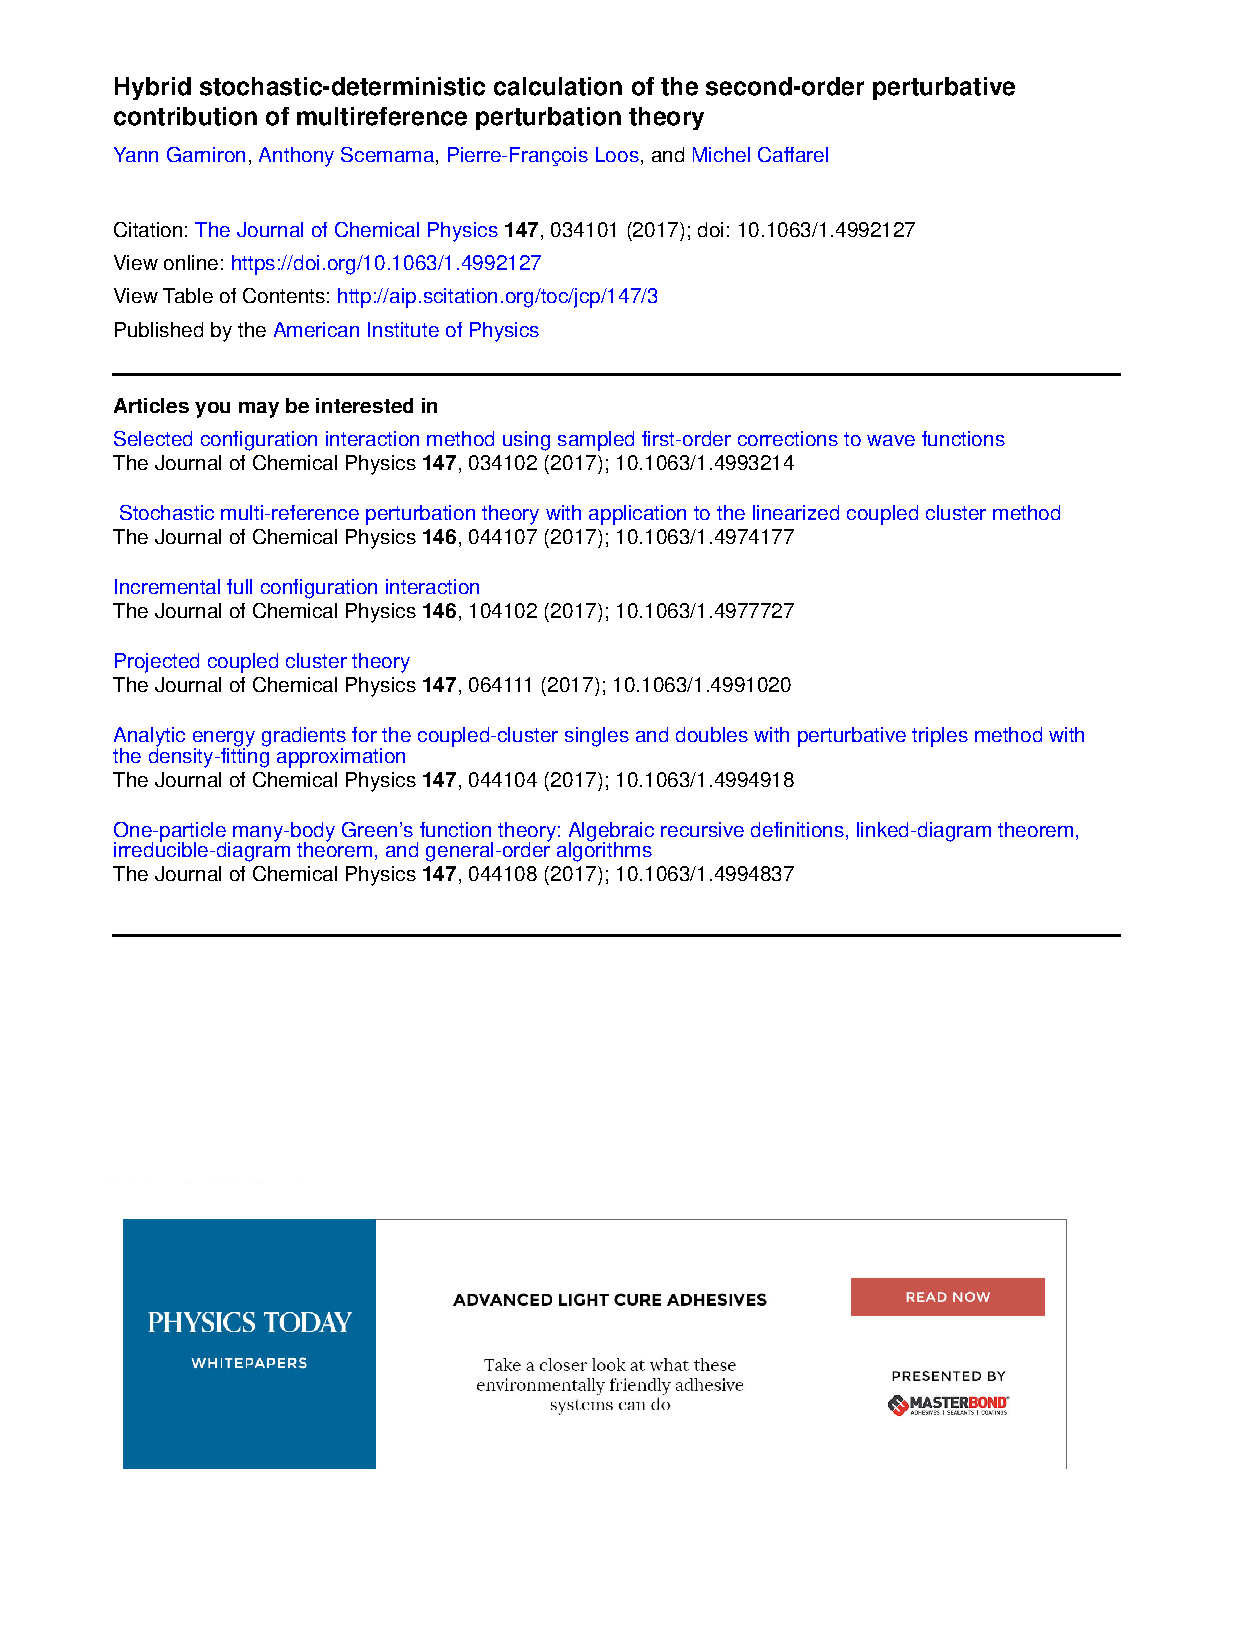
\includepdf[page=2-]{article_pt2}

\end{document}


